\chapter{Lavon Perrin: Mindset, Time Windows, and the Replication Test}

This chapter follows the School of Hard Knocks interview with Lavon Perrin, curated by LazyingArt LLC through Video2Book, as a source-conscious case study in wealth formation. There is no blackboard mathematics in the source. The useful structure is instead practical arithmetic: hours bought by geography, income targets that change plans, a replication test for scale, and a final distinction between money as a number and money as managed freedom.

\section{The Opening Rule: Who You Stand Near}

The episode opens before the formal introduction, with Perrin's mother giving him a rule of proximity. If you stand around nine broke friends, she told him, you are going to be the tenth. If you stand around nine people driving Ferraris, Perrin says, you have a better chance of becoming one of them.

We should read this as an anecdotal rule, not a probability theorem. But it is the first claim in the episode for a reason. Perrin's answer to later questions will keep returning to the same idea: the environment is not decoration around the entrepreneur. It is part of the mechanism.

A compact way to record the claim is:

\begin{equation}
9+1=10.
\end{equation}

The equation is intentionally simple. In Perrin's telling, the tenth person is shaped by the nine people nearby. The content is social rather than algebraic, but the arithmetic gives the reader the hook: repeated exposure has a compounding effect on standards, language, habits, and accepted risk.

\begin{remark}
The transcript later contains garbled car references around Ferraris and Porsches. The notes should preserve the peer-group mechanism while staying cautious about exact car counts unless checked against the video.
\end{remark}

After the cold open, James Doolin introduces the School of Hard Knocks series, ``10 Questions with Millionaires,'' and presents Perrin as the first guest. The first real question is broad: what separates people in business from their peers?

\section{Mindset as the First Tool}

Perrin answers the first question almost immediately: mindset. He says that if he were building a person and could put only one major tool inside that person, it would be mindset.

The order matters. He does not begin with capital, taxes, sales scripts, or product strategy. He begins with interpretation. If a situation is received through the wrong mindset, it looks negative. If the mind is fed mostly negative inputs, such as news he chooses not to watch, then the person has already made the working environment worse before any business decision is made.

\subsection{Question \& Answer}

\paragraph{Question.}
If mindset is the answer, what does it actually change?

\paragraph{Answer.}
In Perrin's answer, mindset changes the first causal step: how a person explains his or her own position. The first object of inspection is not the market but the mirror. If someone is not where they want to be, Perrin says the honest move is to look at oneself and ask what could have been done better.

We can write that as a deliberately modest update rule:

\begin{equation}
\mathrm{result}_{t+1}
=
\mathrm{result}_{t}
+
\mathrm{action}(\mathrm{accountability}_{t},\mathrm{information}_{t}).
\end{equation}

This is not a scientific law. It is a note-writing shorthand for the mechanism Perrin describes. Information diet affects interpretation; accountability changes the next action; the next action changes the next result.

\section{Buying Time With Geography}

Perrin then turns mindset into a concrete operating move. The word in the culture is ``side hustle,'' but the example is sharper than the slogan. Some people on the East Coast, he says, buy a license on the West Coast. That buys them three hours a day.

The arithmetic is the clearest worked example in the interview. The worker keeps the ordinary day: a 9-to-5 job, dinner, perhaps football practice with the kids. Then, when local calling is done around 8 p.m., the West Coast is still available.

\begin{align}
T_{\mathrm{local\ stop}} &= 8{:}00\ \mathrm{p.m.},\\
\Delta_{\mathrm{zone}} &\approx 3\ \mathrm{hours},\\
T_{\mathrm{calling}} &= T_{\mathrm{local\ stop}}+\Delta_{\mathrm{zone}}
                     = 11{:}00\ \mathrm{p.m.}.
\end{align}

So the mechanism is not merely ``work harder.'' It is more precise: extend the reachable market without quitting the job.

\begin{figure}
\centering
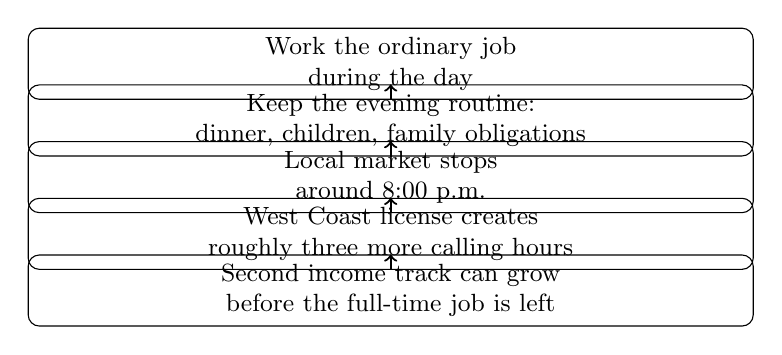
\begin{tikzpicture}[
  node distance=0.72cm,
  every node/.style={font=\small},
  box/.style={
    draw,
    rounded corners,
    align=center,
    text width=0.74\linewidth,
    minimum height=0.82cm
  },
  arrow/.style={->, thick}
]
\node[box] (job) {Work the ordinary job\\during the day};
\node[box, below of=job] (family) {Keep the evening routine:\\dinner, children, family obligations};
\node[box, below of=family] (local) {Local market stops\\around \(8{:}00\) p.m.};
\node[box, below of=local] (west) {West Coast license creates\\roughly three more calling hours};
\node[box, below of=west] (career) {Second income track can grow\\before the full-time job is left};
\draw[arrow] (job) -- (family);
\draw[arrow] (family) -- (local);
\draw[arrow] (local) -- (west);
\draw[arrow] (west) -- (career);
\end{tikzpicture}
\caption{The transcript-backed time-window mechanism: geography turns an evening into a second selling period.}
\end{figure}

This is the first major commercial lesson in the interview. The opportunity is not only in the product. It is in the mismatch between one person's unused time and another market's still-open clock.

\section{The Turn Toward Ownership}

The interviewer next asks about the turning point. Perrin does not give a single dramatic conversion story. He says it was something that ``just kind of happened.'' Corporate America did not feel like a fit. He had questions, he bucked the system, but he was good at sales, people liked him, and he could lead.

\subsection{Question \& Answer}

\paragraph{Question.}
Was there one decisive turning point?

\paragraph{Answer.}
Not in the clean, cinematic sense. Perrin describes accumulation. He learned tools from other companies, then wanted to put those tools into action for himself. The car business gave him another pressure: he did not want the lifestyle he associated with that world, and he wanted to see his kids.

So ownership appears as a structural solution to a personal constraint. The point is not just ``be your own boss.'' It is: choose a structure that allows the work, the family constraint, and the desired operating style to coexist.

We can summarize the transition as:

\begin{equation}
\mathrm{employment\ learning}
+
\mathrm{personal\ constraint}
\longrightarrow
\mathrm{ownership\ attempt}.
\end{equation}

Again, the arrow is not a universal law. It is the local mechanism in Perrin's account.

\section{Scaling by Raising the Target and Testing the Operator}

The next question asks what enabled Perrin to scale. He begins with numbers. Everyone wants to make \(\$100{,}000\) a year, he says, but if the plan were to make \(\$500{,}000\), then even failing at that larger goal might still leave a person near \(\$100{,}000\).

\begin{equation}
G_{\mathrm{common}}=\$100{,}000,\qquad
G_{\mathrm{plan}}=\$500{,}000,\qquad
G_{\mathrm{plan}}=5G_{\mathrm{common}}.
\end{equation}

The claim should be handled carefully. Perrin is not proving that a larger target mechanically produces more income. He is saying that target size changes the plan. A small target can permit a small operating design. A larger target demands a different one.

\subsection{Question \& Answer}

\paragraph{Question.}
Why would a larger goal change the result?

\paragraph{Answer.}
Because the plan must be built to match the goal. A \(\$100{,}000\) wish may require one pattern of behavior. A \(\$500{,}000\) plan asks different questions about volume, skill, accountability, and repeatability. Perrin's point is not that failure is desirable; it is that aiming at a larger structure may produce a higher fallback than aiming at the fallback directly.

His second scaling test is more personal: would the company or the people he does business with be happy if they had ten of him?

\begin{equation}
N_{\mathrm{copies}}=10.
\end{equation}

This is a useful operator test. One reliable operator creates income. Ten reliable operators suggest scale. But if the answer to the ten-copy question is no, the problem is not yet scale; the problem is quality of the unit being scaled.

\begin{table}
\centering
\begin{tabular}{|p{0.42\linewidth}|p{0.42\linewidth}|}
\hline
\textbf{Test} & \textbf{What It Measures} \\
\hline
\(\$100{,}000\) wish & A common desired outcome, often without a large enough plan. \\
\hline
\(\$500{,}000\) plan & A larger operating design that may change behavior even if the goal is missed. \\
\hline
Ten-copy question & Whether the current operator is reliable enough to replicate. \\
\hline
\end{tabular}
\caption{Perrin's scale logic: raise the target, then test whether the operator is worth multiplying.}
\end{table}

After this, Perrin returns to environment. He talks about surrounding himself with successful people, moving downtown, and being around people living the lifestyle he wanted. The opening rule has now become part of the scale section. The people nearby are not just friends; they are a reference class.

\section{Risk, Sales, and Personal Development}

The interviewer then asks about risk. Perrin answers bluntly: there is no success without risk. But the word ``risk'' in his answer is not recklessness. He says the risk must be calculated, learned from, and paired with self-belief and education.

The implicit update rule is:

\begin{equation}
\mathrm{risk}_{\mathrm{useful}}
=
\mathrm{calculation}
+
\mathrm{learning}
+
\mathrm{commitment}.
\end{equation}

Then the interview turns to sales in 2022. Perrin's answer is again not a trick script. It is personal development. He says he did not read much in his youth or after college, though he did take online classes in the early 2000s and earned his degree. Later, personal development helped him validate thoughts and ambitions that he already had but had not understood.

The numerical marker is small but important:

\begin{equation}
B_{\mathrm{last\ year}}\approx 15\ \mathrm{books}.
\end{equation}

He names three books: \textit{Think and Grow Rich} by Napoleon Hill, \textit{Rich Dad Poor Dad}, and \textit{Go for No}. The first stands above the others in his account. His mentor rereads it every September, and Perrin is preparing to read it again as well.

\begin{remark}
The book list should be preserved as named evidence, not generalized into an abstract reading recommendation detached from Perrin's story.
\end{remark}

\section{Mistakes, Time, and What Money Is For}

The late part of the interview gathers several practical limits. The biggest challenge in business ownership, Perrin says, is learning how to be a business owner: consistency, budgeting, knowing where money goes, and accepting ups and downs. He also names the danger of overanalysis. People can analyze a situation so long that they do not move.

When asked about his worst financial decision, he resists the premise. He does not want to treat every bad outcome as a pure negative. He compares it to sports: you do not necessarily lose; you learn. Then he gives a concrete story. He had long wanted a BMW 750, partly because he grew up mainly in Germany. He had the opportunity to own two. A mechanic in Austin had warned him that if he bought one, they would become good friends because he would see the mechanic often. Perrin concludes that he might still be glad he did it, but he should have done it with a maintenance plan and better preparation.

The work-life balance answer shifts from balance to time leverage. Perrin argues that everyone has the same number of hours, so the difference is how time is handled and who is placed around the work. He invokes the familiar rule: go alone if you want to go fast; go with others if you want to go far.

\subsection{Question \& Answer}

\paragraph{Question.}
Does money buy happiness?

\paragraph{Answer.}
Perrin narrows the question. Money can buy freedom, he says, if a person knows what to do with it. But a million dollars does not solve the management problem. If someone cannot manage a thousand dollars, he says, that person cannot manage a million dollars.

\begin{equation}
\$1{,}000{,}000 = 1000 \times \$1{,}000.
\end{equation}

This equation is not offered as financial theory. It is a discipline test. A larger number magnifies the same habits. In Perrin's account, freedom is not purchased by the amount alone; it is purchased by the combination of money and the ability to handle money.

\begin{figure}
\centering
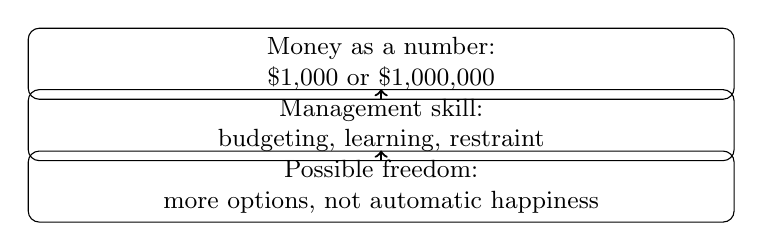
\begin{tikzpicture}[
  node distance=0.78cm,
  every node/.style={font=\small},
  box/.style={
    draw,
    rounded corners,
    align=center,
    text width=0.72\linewidth,
    minimum height=0.78cm
  },
  arrow/.style={->, thick}
]
\node[box] (money) {Money as a number:\\\(\$1{,}000\) or \(\$1{,}000{,}000\)};
\node[box, below of=money] (skill) {Management skill:\\budgeting, learning, restraint};
\node[box, below of=skill] (freedom) {Possible freedom:\\more options, not automatic happiness};
\draw[arrow] (money) -- (skill);
\draw[arrow] (skill) -- (freedom);
\end{tikzpicture}
\caption{Perrin's final distinction: money can buy freedom only when money is managed.}
\end{figure}

\section{Summary}

The episode begins and ends with management of surroundings: who is nearby, what information enters the mind, which market is still open, whether the operator is worth copying, and whether money is handled before it is multiplied. Perrin's claims are practical rather than formal. The mathematics is therefore bookkeeping mathematics, but it is still useful: \(8{:}00+3=11{:}00\), \(\$500{,}000=5\times\$100{,}000\), \(N_{\mathrm{copies}}=10\), \(B\approx15\), and \(\$1{,}000{,}000=1000\times\$1{,}000\).

The durable lesson is not that wealth follows a formula. It is that Perrin keeps converting slogans into operating tests. Mindset becomes accountability. Side hustle becomes a three-hour market window. Scale becomes a ten-copy question. Risk becomes calculated learning. Money becomes freedom only when the smaller amount is already being managed.